\documentclass{koala-en}
\usepackage[english]{babel}
\usepackage{lastpage}
\usepackage{pdfpages}
\renewcommand{\arraystretch}{1.5} %% Aeration des tableaux
\hyphenpenalty 10000
\usepackage{fancyhdr}
\usepackage{fmtcount}
\pagestyle{fancyplain}
\fancyhf{}
\renewcommand{\chaptermark}[1]{\markboth{#1}{}}
\renewcommand{\sectionmark}[1]{\markright{#1}}
\renewcommand{\headrulewidth}{0.8pt}
\renewcommand{\footrulewidth}{0.8pt}
\fancyhead[R]{\nouppercase{\leftmark}}
\lfoot{Camille Gardet - Internship report - August 2014}
\rfoot{\thepage/\pageref{LastPage}}
\setcounter{secnumdepth}{5}
\setcounter{tocdepth}{5}
\newcommand*{\glossaryname}{Dictionary}
\usepackage{glossaries}
\newcommand{\dictentry}[2]{%
  \newglossaryentry{#1}{name=#1,description={#2}}%
  \glslink{#1}{#1*}%
}
\makeglossaries

%%%%%%%%%%%%%%%%%%%%%%%%%%%%%%%%%%%%%%%%%%%%%%%%

\begin{document}

\title{Internship report}
\subtitle{CS - from  May, \ordinalnum{5} to October, \ordinalnum{7}}

\member{Camille Gardet - }{camille.gardet@epitech.eu}

\summary
{
  This document contains three distinct sections, written in english, intended for three different kind of person :
  \begin{itemize}
     \item A part for a newcomer in the company will resume / continue / maintain the project in which I was involved.
     \item A part to convince my internship supervisor to fit into the team of a new project that I am particularly interested in.
     \item A part to convince a high supervisor (non-technical) to entrust you with the full responsibility for a project, from start to finish, with customer contacts.
  \end{itemize}
  Word with a star in its right upper corner is defined in the glossary at the end of this document. It's clickable (only for numeric version, should I precise this ?).
}

\maketitle

\newpage
\thispagestyle{empty}

\tableofcontents

\thispagestyle{fancy}
\newpage

\part{Documentation for a newcomer}
\chapter{Company presentation}
\section{Sector}
CS is an international company specialized in critical systems of the defense market, security, space, aeronautics and energy.

\begin{figure}[!ht]
  \center
  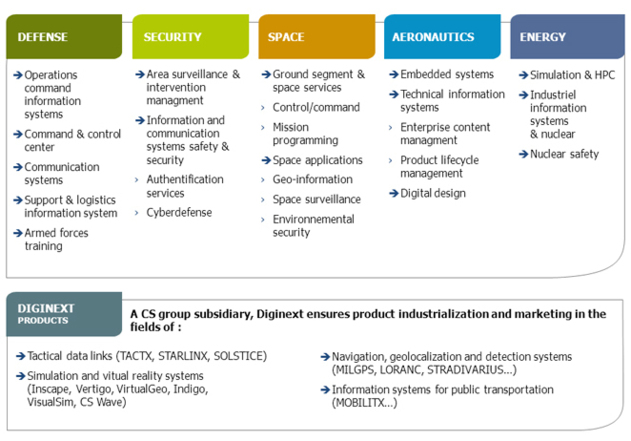
\includegraphics{market.jpg}
  \caption{Critical sectors}
\end{figure}

CS is now a leader in the field of air traffic control. Diginext, a subsidiary of the company, is a leader in \emph{\dictentry{Link 16}{A military tactical data exchange network used by US and NATO. Its specification is part of the family of Tactical Data Links}} and military data links.

\section{Company}
Located in France, Germany, Croatia, Romania, United-Kingdom, Chile, Canada, Emirates, US, Puerto Rico, CS acts all around the world.

\begin{figure}[!ht]
  \center
  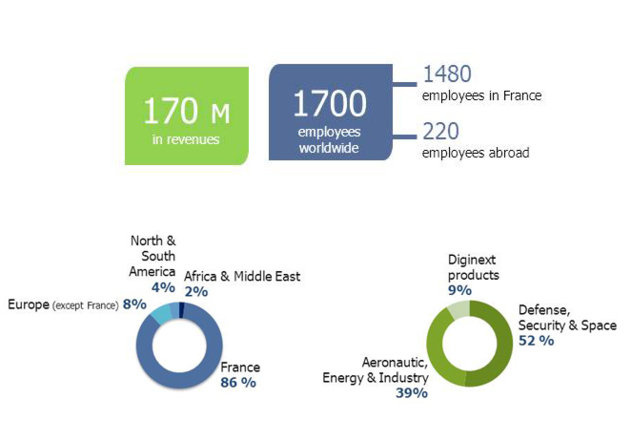
\includegraphics{revenue.jpg}
  \caption{International partners and turnover allocation}
\end{figure}

The company is in partnership with top-notch industrial and commercial company like EADS and Cegelec for air operations, Intel and Wolfram for high performance consulting, Sopra for logistics information systems.

\thispagestyle{fancy}
\newpage

\section{Business unit}

\begin{figure}[!ht]
  \center
  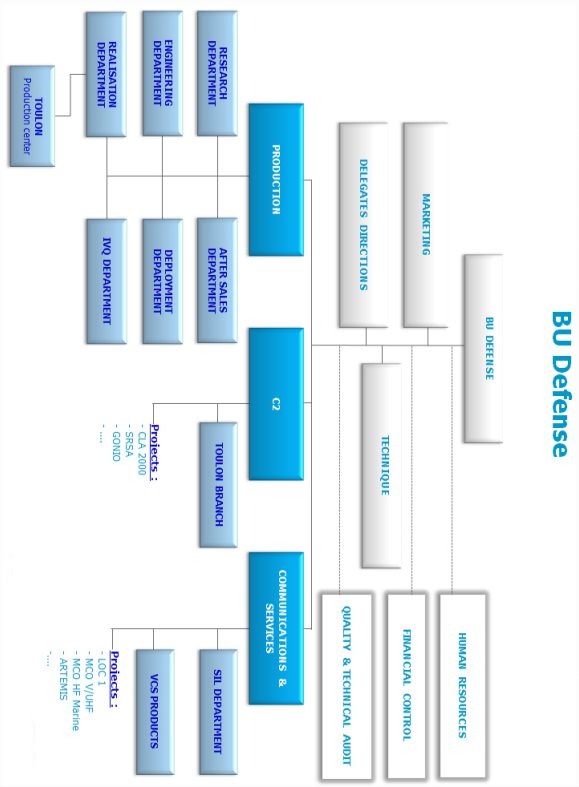
\includegraphics[width=15cm]{ochart.png}
  \caption{Organization chart of the Defense Business Unit}
\end{figure}

The mission of the Defense unit is to implement solutions that meet the internal and external security needs, design and integrate command centers to collect, share and view in real time all the information needed for planning and driving joint army operations.

\section{Contextualization}
CS has had the dual experience, on the one hand of developing security components and solutions, and on the other hand, of managing several e-administration and e-transaction projects. Moreover, backed by its expertise in cryptography and public-key infrastructures, CS offers a complete range of security applications: encryption and implementation in networking equipment, identification and validation, non-reversible transactions, data and interchange confidentiality, secured application flows, and rights management and attribution.
\newline
\newline
In January 2012, CS acquires \emph{Prelude-IDS}, an open-source \dictentry{SIEM}{Security Information \& Event Management - Provide real-time analysis of security alerts generated by network hardware and applications}, and puts a lot of effort to rebuild it, and puts it back online.

\thispagestyle{fancy}
\newpage

\chapter{Prelude}
\section{Definition - What is Prelude ?}

\begin{figure}[!ht]
  \center
  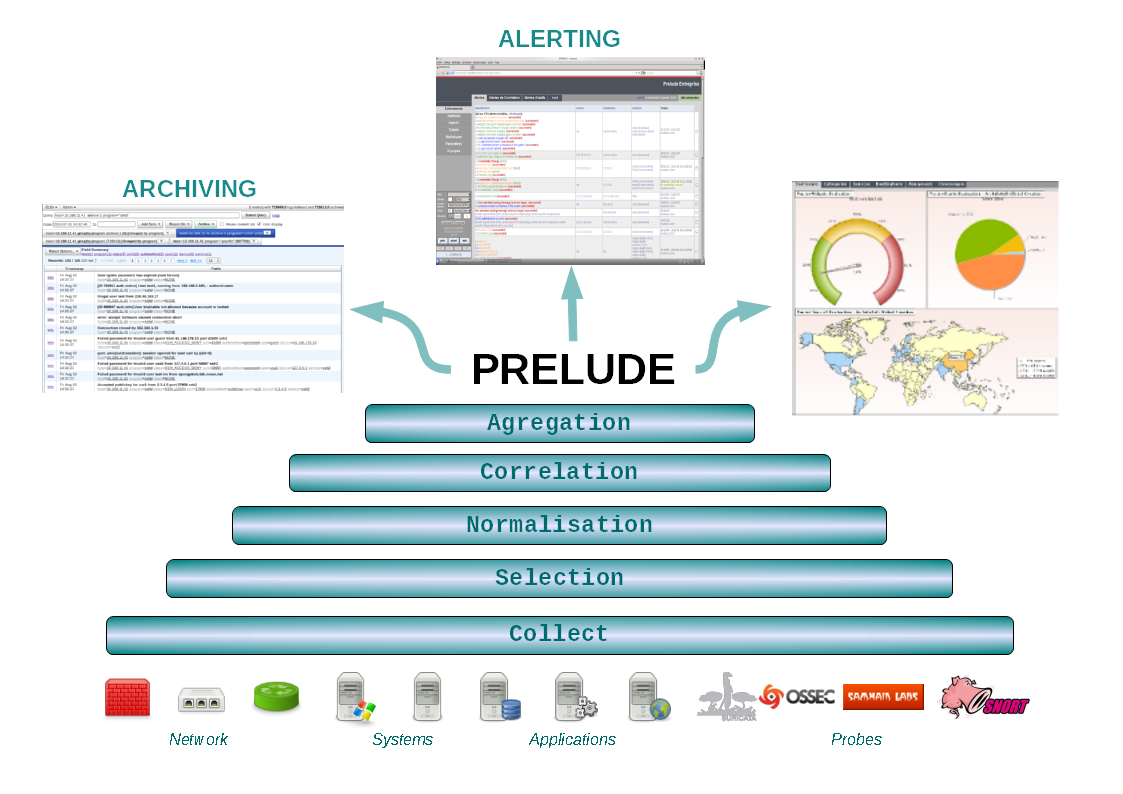
\includegraphics[width=15cm]{archi-simple.png}
  \caption{General overview}
\end{figure}

Prelude is a universal \emph{Security Information \& Event Management} (\dictentry{SIEM}{Security Information \& Event Management - Provide real-time analysis of security alerts generated by network hardware and applications}) system. Prelude collects, normalizes, sorts, aggregates, correlates and reports all security-related events independently of the product brand or license giving rise to such events.
\newline
\newline
As well as being capable of recovering any type of log (system logs, syslog, flat files, etc.), Prelude benefits from a native support with a number of systems dedicated to enriching information even further (snort, samhain, ossec, auditd, etc.).
\newline
\newline
Security events are normalized thanks to a single format, called the \emph{Intrusion Detection Message Exchange Format} (\dictentry{IDMEF}{Intrusion Detection Message Exchange Format - define data formats and exchange procedures for sharing information of interest to intrusion detection and response systems and to the management systems that may need to interact with them}), which is an international standard created upon the initiative of \dictentry{IETF}{Internet Engineering Task Force - develops and promotes voluntary Internet standards} along with the participation of Prelude teams to enable interacting with the various security tools currently available on the market.


\section{How does it work ?}

\begin{figure}[!ht]
  \center
  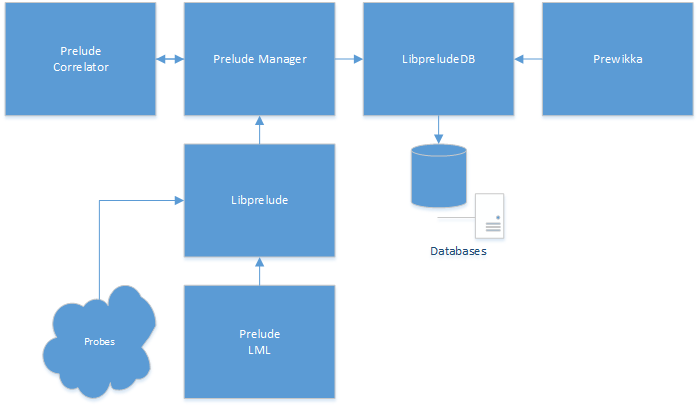
\includegraphics[width=15cm]{prelude.png}
  \caption{Communication between elements}
\end{figure}

\emph{Prelude LML} monitors system activites and read logfile generated by any kind of probes and create \dictentry{IDMEF}{Intrusion Detection Message Exchange Format - define data formats and exchange procedures for sharing information of interest to intrusion detection and response systems and to the management systems that may need to interact with them} alerts with \emph{Libprelude}.
\newline
\newline
\emph{Libprelude} is a library used to make \dictentry{IDMEF}{Intrusion Detection Message Exchange Format - define data formats and exchange procedures for sharing information of interest to intrusion detection and response systems and to the management systems that may need to interact with them} alerts and agent, to connect to a data bus (here, \emph{Prelude Manager}).
\newline
\newline
\emph{Prelude Manager} is a server with secured connections, which receives alerts and write it on any kind of support, like databases or files.
\newline
\newline
\emph{LibpreludeDB} is an abstraction to interface the manager with any kind of databases (pgsql, mysql, sqlite).
\newline
\newline
\emph{Prelude Correlator} is a correlation factory, which is allowed to create new alert based on multiple alert.
\newline
\newline
\emph{Prewikka} is the GUI of Prelude. Web-based, it shows alerts, correlated alerts, probes states, statistics about systems, alerts, and so on.

\chapter{Latest developments - Documentations}
Prelude is an old and open-source based project without any user or developer documentations.
\newline
\newline
A part of the mission involve to write these documentations, helped with the reference document of CS :
\begin{itemize}
  \item System/Subsystem Specification (SSS) - The requirements to be met by the system,
  \item System/Subsystem Design Description (SSDD) - The design of the system
\end{itemize}

Each module of Prelude must be covered. \emph{Libprelude} documentation is already written and will be used as example in this document. Guidelines to write these documents are provided below.

\thispagestyle{fancy}
\newpage

\section{System/Subsystem Specification (SSS)}
\subsection{Needs}
Understanding the needs is the first thing to know and answer questions like \emph{Why do I need this ?} or \emph{How can I fulfill this requirements ?}. The requirements are submited by the client, most of time, but also by CS, to match a local standard.

\subsection{Technical requirements}
\emph{How things should work ?}
\newline
While being general, each features of a module are formated as a requirement, describing its operating.
A small flow-chart to illustrate this is strongly recommended.

\begin{figure}[!ht]
  \center
  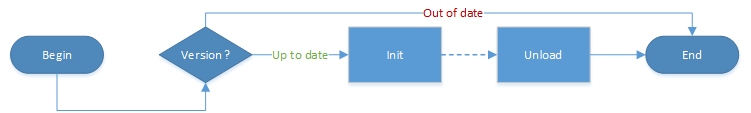
\includegraphics[width=15cm]{sss.png}
  \caption{Init Libprelude - How should it proceeds}
\end{figure}

Followed by :
\begin{lstlisting}
  LIB_USE_VERSION : Check library version
  How : Use a function to return the version
  Why : The version can be checked before the initialisation

  ...
\end{lstlisting}
Same for the init and unload part.

\subsection{External interface requirements}
\emph{What will provide external connection ?}
\newline
Not only network of course. Everything that will communicate/use/connect to the module is an external interface.
It can be other module of the project, external library, \dictentry{API}{Application Programming Interface - specifies how some software components should interact with each other}, language binding, etc.

\subsection{Internal interface requirements}
\emph{What use my module to run properly ?}
\newline
If the module use a configuration file, or data in a specified standard format, it should be listed as an internal interface. For example, the IDMEF format is specified in a \dictentry{RFC}{Request For Comments - the principal technical development and standards-setting bodies for the Internet}.

\subsection{Environment requirements}
Everything environment related, like \emph{Should my library be crossplatform ?} or \emph{What happens when my system reboot ?}.

\subsection{Definition and conception constraints}
Languages or tools that \textbf{must} be used to implement the module. \emph{Libprelude} must be written in C for example.

\thispagestyle{fancy}
\newpage

\section{System/Subsystem Design Description (SSDD)}
\subsection{Design principle}
For each main part of the module, a description about the way it will be designed should be made. It can be data exchange, communication channel or error and configuration management.

\subsection{Software structure}
\emph{What is the internal structure ?}
\newline
It can be a tree view, with details about folders, what it contains, why is it used. Third party library are also mentioned here, with proper explanations given on its usage.

\subsection{System operating}
The huge part. The scale is the function, what does it do and how, and such, for each function in each part of the module. A flow-chart is highly recommended.
\newline
\newline
Short example for \emph{Libprelude} and the function to initialise the library :

\begin{figure}[!ht]
  \center
  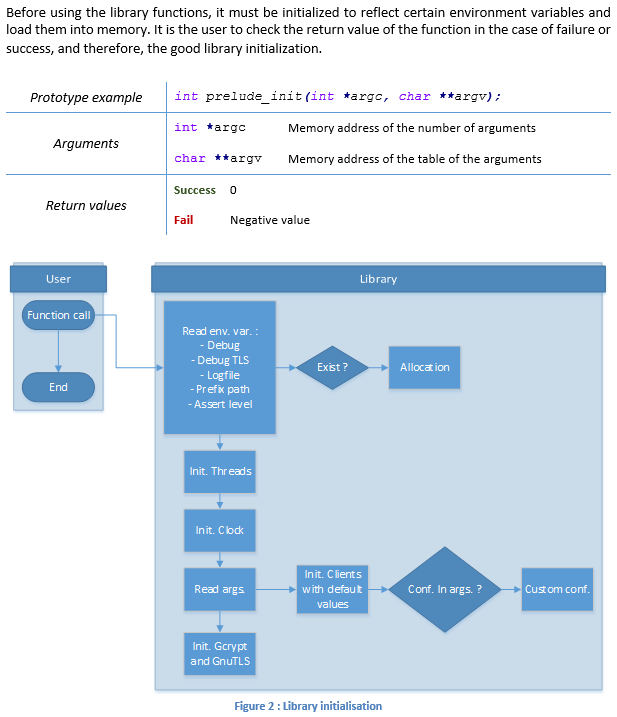
\includegraphics{sysop.png}
  \caption{Description of the library init function in Libprelude}
\end{figure}

\thispagestyle{fancy}
\newpage

\chapter{Latest developments - Coding}
\section{CS standard}
To develop features on Prelude, it's recommended to use :
\begin{itemize}
  \item CentOS 6 virtual machine,
  \item Python 2.6,
  \item C, standard C89,
  \item Redmine, for project management and bug-tracking tool,
  \item Latest version of Prelude, found on \url{http://www.prelude-ids.org}
\end{itemize}

\section{A new probe, Motion}
Using a webcam, the probe should be able to raise alert when it detects movement. \emph{How ?}
\subsection{Motion ?}
Motion is a small tool to monitor video streams, coming from one or many video device and is able to detect movement.
\newline
\newline
The tool is written in C for linux based OS.
\newline
\newline
Since its version 3.1.12, the tool is maintained by Kenneth Lavrsen and a small community.
\newline
Homepage : \url{http://www.lavrsen.dk/foswiki/bin/view/Motion/WebHome}

\subsection{Implementation}
The motion source code is well commented. It is easy to navigate in.
\newline
\newline
The files \emph{motion.c} and \emph{motion.h} contains the code where a movement is detected. An alert should be raised from these files.
\newline
\newline
Motion use a structure \emph{context} which includes the whole software configuration during its execution, and the last recorded pictures.
Prelude initialisation is done at this structure initialisation :
\begin{lstlisting}
  AlertPreludeCtx *prelude_ctx = AlertPreludeInitCtx();
  cnt->prelude_context = prelude_ctx;
\end{lstlisting}
The function \emph{AlertPreludeInitCtx()} initialise a Prelude context.
\newline
\newline
The function \emph{motion\_loop()} is a infinite loop to capture the video stream, and detect a movement. The alert-raising code is inserted :
\begin{lstlisting}
  AlertPrelude(cnt->prelude_context, cnt->current_image);
\end{lstlisting}
The function \emph{AlertPrelude()} create and send an alert to the \emph{Prelude Manager} with the current image as extra data, to display it for example.

\subsection{Results}
After registering Motion in Prelude and running it, it appears as a probe in \emph{Prewikka}.
\begin{figure}[!ht]
  \center
  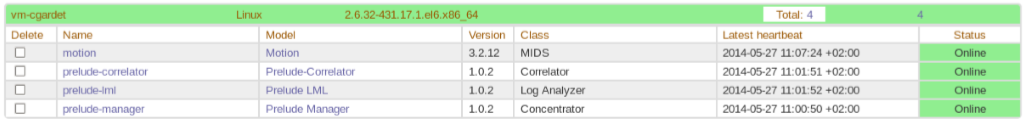
\includegraphics[width=15cm]{motionprobe.png}
  \caption{Motion as a probe in Prewikka}
\end{figure}

And it generates some alerts as well.
\begin{figure}[!ht]
  \center
  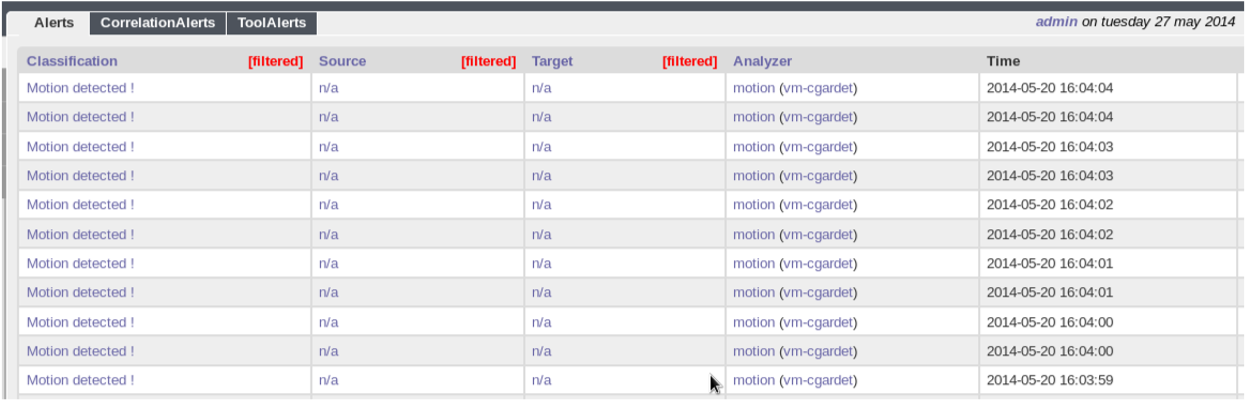
\includegraphics[width=15cm]{motionalerts.png}
  \caption{Alerts raised by Motion in Prewikka}
\end{figure}

\thispagestyle{fancy}
\newpage

\section{Enhance statistics in Prewikka}
Create new visualisation graph to diversify statistics / forensics.
\subsection{One library, to rule them all}
Old graph are Adobe Flash based, an ageing technology.
\newline
\newline
Instead, Javascript is recommended in this case and already used in \emph{Prewikka}. After a small research, the library \textbf{D3.js} seems to fulfill all the needs.
\newline
\newline
\emph{D3} binds arbitrary data to a Document Object Model (DOM), and then apply data-driven transformations to the document. For example, \emph{D3} generates an HTML table from an array of numbers. Or, use the same data to create an interactive SVG bar chart with smooth transitions and interaction.
\newline
\newline
Homepage : \url{http://d3js.org/}
\newline
Example gallery : \url{https://github.com/mbostock/d3/wiki/Gallery}

\subsection{Implementation}
For any graphes, the first step is to create a standalone version, working offline, supplied from a CSV data file. Data can be IDMEF fields like :
\begin{lstlisting}
``IP Source'', ``IP Target'', ``Assessment'', ``Analyzer'', ``Date''
``10.10.10.3'',''232.136.239.176'',''Bruteforce'',''Prelude-LML'',''24/02/2005T11:45''
``10.10.10.20'',''193.227.171.216'',''SSH Failed'',''Snort'',''09/02/2005T14:59''
``10.10.10.16'',''106.190.182.175'',''SSH Failed'',''OSSEC'',''09/10/2007T09:06''
\end{lstlisting}

Each line is an alert. A python script is provided in appendix to generate this kind of file.
\newline
\newline
Once the graphe works, the integration in \emph{Prewikka} can begin. It means :
\begin{itemize}
  \item Templating - HTML code,
  \item Create view - Setting up data to fill the template,
  \item Fetch database - Collecting alerts from the database, and not from a file
\end{itemize}

Features already provided by \emph{Prewikka} must be kept, as filtering by date, event, etc.

\thispagestyle{fancy}
\newpage

\subsection{Results}
As example, a \dictentry{Circos}{Kind of graphe to visualize data in a circular layout, ideal for exploring relationships between objects or positions. Homepage : \url{http://circos.ca/}}-like in D3.js.

\begin{figure}[!ht]
  \center
  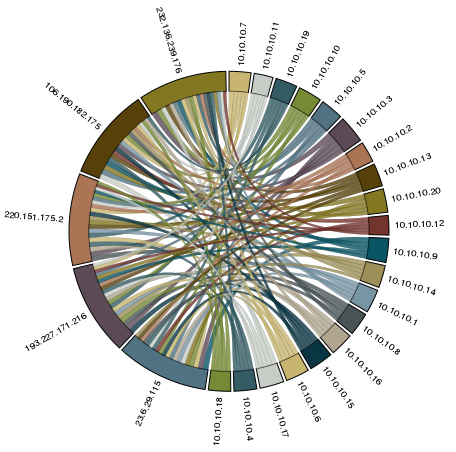
\includegraphics[width=15cm]{circos.png}
  \caption{Standalone version of a Circos-like graphe}
\end{figure}


We can add information about the data.

\begin{figure}[!ht]
  \center
  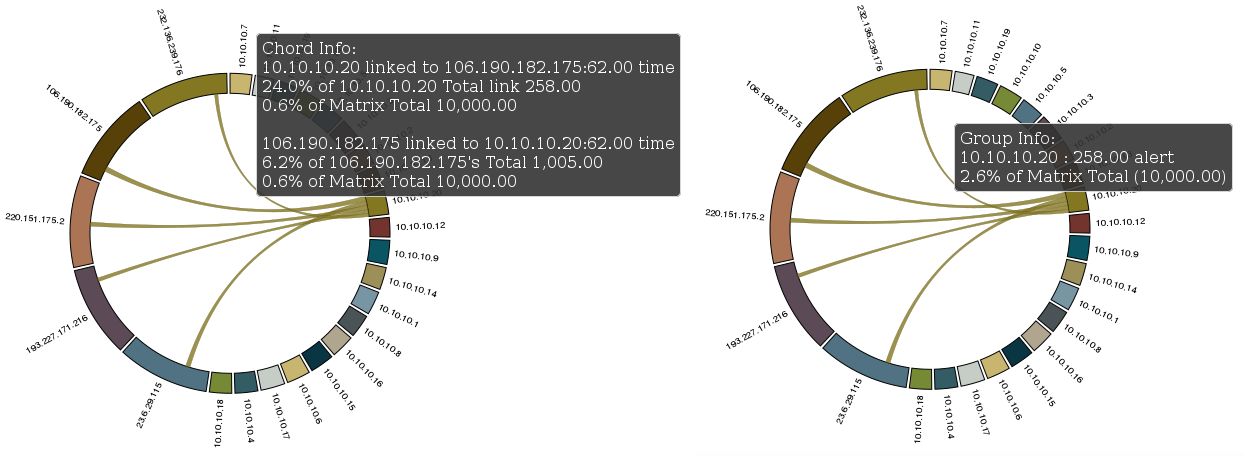
\includegraphics[width=15cm]{circostt.png}
  \caption{More information about links}
\end{figure}

\thispagestyle{fancy}
\newpage

The merge in \emph{Prewikka} with the filters can be done.

\begin{figure}[!ht]
  \center
  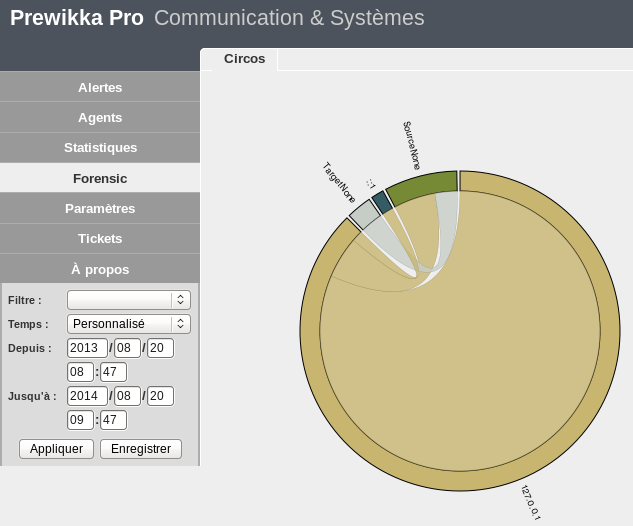
\includegraphics[width=15cm]{circosprew.png}
  \caption{The graphe in \emph{Prewikka}}
\end{figure}

Applying filters update the chart in real-time.

\thispagestyle{fancy}
\newpage

\section{Make GeoIP customisable}
\subsection{GeoIP ?}
\emph{GeoIP} enables the identification, the location, organization, connection speed, and user type of IP address. The GeoIP databases are among the most popular and accurate IP geolocation databases available.
\newline
\newline
Homepage : \url{https://www.maxmind.com}
\newline
\newline
It is used in \emph{Prelude} to locate the source of an alert.
\subsection{Implementation}
\emph{Customisable ?}
Actually, only public IP addresses can be identified, which is how the tools performs. It might be possible to create custom IP range and associate them to a custom location.
\newline
\newline
\emph{How GeoIP works ?}. Range of IP are stored in a database and linked to a location. E.g. : 2.0.0.0 to 2.15.255.255 are reserved to \emph{France Telecom}. With this, it is easy to compare and get the location name of a determined IP. The IP database used is highly optimized, not directly readable and \emph{Maxmind} does not provide tools to modify it. So, the principle is finding a way to decypher it, insert custom range, and re-cypher it. However, the database exists in a CSV file format, avoiding the decyphering step, and implying a regeneration of the database binary formated.
\newline
\newline
Same process as the graphes, a view and a template must be created. The view is a simple HTML form with the necessary fields to fill up a custom range. The view is python code to parse the GeoIP CSV file and store it in a dictionnary. The file is provided in the appendix.

\subsection{Results}
As seen below, the form displays :
\begin{itemize}
  \item ``Create a range'', to create a location with its long name, associate to a two letters short name,
  \item ``Select a range'', load or delete existing range. The loaded range displays IP in the field ``IP range'',
  \item ``IP range'', shows all IP range of the location, with the possibility to massive deletion/insertion and submit modification,
  \item ``export to GeoIP binary file'', converts the CSV file format to binary database, used by all the API provided by \emph{Maxmind}
\end{itemize}

\begin{figure}[!ht]
  \center
  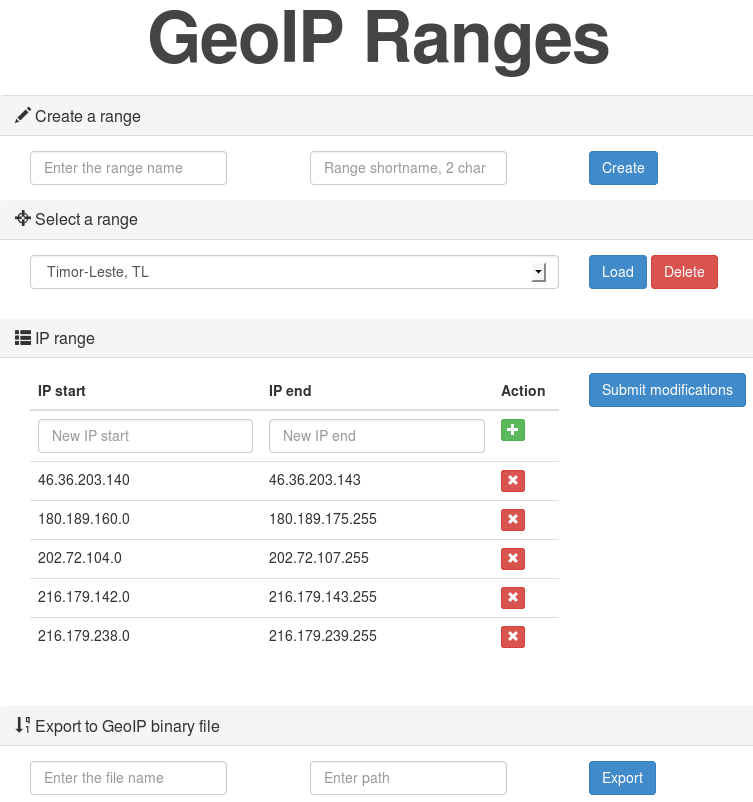
\includegraphics[width=15cm]{geoip.png}
  \caption{The form to create/edit/delete GeoIP range}
\end{figure}

\chapter{Final word}

\thispagestyle{fancy}
\newpage

\chapter{Appendix}

All of the files can be viewed on \url{https://github.com/M3nace/Prelude}

\section{Python script to generate alert}
\begin{lstlisting}
#!/usr/bin/env python3
"''
Generate alert and store them in a CSV file, formated like :
``target'', ``source'', ``classification'', ``analyzer'', ``date'',
    ^           ^               ^                ^            ^
    |           |               |                |            |
    |           |               |                |            --------- The date of the alert, format : DD/MM/YYYYTHH:MM
    |           |               |                |
    |           |               |                ------------------- Analyzer name, which create the alert
    |           |               |
    |           |               ----------------------------------- Type of the alert
    |           |
    |           ------------------------------------------------ IP of the device which create the alert
    |
    ---------------------------------------------------------- IP of the device which has been targeted

Contiguous IP are generated with the function ipRange(start, end), to simulate a targeted network.
Where ``start'' is the first IP in the range and ``end'', the last. Both type are strings.
E.g. : ipRange(``192.168.1.0'', ``192.168.1.5'') will return a list including :
[ ``192.168.1.0'', ``192.168.1.2'', ``192.168.1.3'', ``192.168.1.4'', ``192.168.1.5'' ]

Random date are generated with the function randomDate(start, end), to simulate attacks on a period of time.
Where ``start'' is the beginning of a period, and ``end'', the end of it. Both type are datetime.

IP Source are randomly generated and stored in a list.
Classification and analyzer are randomly picked from an established list. Lazy, I know.

And finally, the CSV is written, line by line, picking a ``random'' settings each loop. ``Random'' because
the random module should be called ``pseudo-random'':
> Generate 5000 alerts.
> You have a list of 5 analyzers.
> You will have a CSV where each analyzer appears around 1000 times.
> That's not a place to talk about that.
"''

import os
import sys
import random
import csv
import json
import time
from datetime import timedelta
from datetime import datetime
from random import randint

# How many IP source do you want ?
nb_ip_source = 5
# How many alert (line in the CSV file) do you want ? /!\ The higher, the harder to compute (for the diagram) /!\
nb_alert = 5000

def ipRange(start_ip, end_ip):
   start = list(map(int, start_ip.split(``.'')))
   end = list(map(int, end_ip.split(``.'')))
   temp = start
   ip_range = []

   ip_range.append(start_ip)
   while temp != end:
      start[3] += 1
      for i in (3, 2, 1):
         if temp[i] == 256:
            temp[i] = 0
            temp[i-1] += 1
      ip_range.append(``.''.join(map(str, temp)))

   return ip_range


def randomDate(start, end):
   return (start + timedelta(seconds=randint(0, int((end - start).total_seconds())))).strftime('%d/%m/%YT%H:%M')#.date()


def main(argv=None):
   target_list = ipRange(``10.10.10.1'', ``10.10.10.20'')
   source_list = [ ]
   classification_list = [ ``SSH Failed'', ``Bruteforce'', ``DDoS'', ``Eth. Sniffing'', ``Buffer overflow'' ]
   analyzer_list = [ ``Prelude-LML'', ``Suricata'', ``OSSEC'', ``Samhain'', ``Snort'' ]
   date_begin = datetime.strptime(``01 Jan 00'', ``%d %b %y'')
   date_end = datetime.strptime(``31 Dec 14'', ``%d %b %y'')
   # We list the index here, to write it on the first line of the CSV file
   indexes = [``target'', ``source'', ``classification'', ``analyzer'', ``date'']

   for j in range(nb_ip_source):
      source_list.append('.'.join('%s'%random.randint(0, 255) for i in range(4)))

   with open('alert.csv', 'w') as csvfile:
      spamwriter = csv.writer(csvfile, delimiter=',', quotechar='''', quoting=csv.QUOTE_ALL)
      spamwriter.writerow(indexes)
      for i in range(nb_alert):
         spamwriter.writerow([random.choice(target_list),
                              random.choice(source_list),
                              random.choice(classification_list),
                              random.choice(analyzer_list),
                              randomDate(date_begin, date_end)])

   return 0

if __name__==''__main__'':
   status = main()
   sys.exit(status)
\end{lstlisting}

\section{Python script to parse GeoIP CSV file}
\begin{lstlisting}
#!/usr/bin/env python

"''
CSVReader - Read a data.cvs GeoIP format file and store it in a dictionary
The CVS format parsed must match the GeoIPCountryWhoIs.cvs :
``IP Start'', ``IP End'', ``IP Start INT format'', ``IP End INT format'', ``Short Name'', ``Range Name''
    -> IP Start/End : the first/last ip of the range
    -> IP Start/End INT format : Same as IP start, but in int format (see below)
    -> Short Name : Abreviation for the range name
    -> Range Name : Full range Name
Example : ``192.168.1.0'', ``192.168.1.255'', ``3232235776'', ``3232236031'', ``SN'', ``Small Network''

IP int calculation :
(first octet * 256^3) + (second octet * 256^2) + (third octet * 256) + (fourth octet)
For 192.168.1.0 :
    (192 * 256^3) + (168 * 256^2) + (1 * 256) + (0)
<=> 3221225472 + 11010048 + 256
<=> 3232235776

The dictionary keys are the tuple (Range Name, Short Name)
The items are a list of as many tuple as IP range for the key
Example :
(Private Network, PN)
[
    (``10.0.0.0'', ``10.255.255.255'', ``167772160'', ``184549375''),
    (``172.16.0.0'', ``172.31.255.255'', ``2886729728'', ``2887778303''),
    (``192.168.0.0'', ``192.168.255.255'', ``3232235520'', ``3232301055'')
]

(My Network, MN) [(``127.3.0.0'', ``127.3.255.255'', ``2130903040'', ``2130968575'')]
"''

import csv
import collections

class CSVReader:
    def __init__(self, csv_file):
        self.csv_file = csv_file
        self.db = { }

    def parse_file(self):
        with open(self.csv_file, 'r') as fd:
            reader = csv.reader(fd)
            for row in reader:
                ip_start, ip_end, ipint_start, ipint_end, short_name, range_name = row
                if (range_name, short_name) in self.db:
                    self.db[(range_name, short_name)] += [(ip_start, ip_end, ipint_start, ipint_end)]
                else:
                    self.db[(range_name, short_name)] = [(ip_start, ip_end, ipint_start, ipint_end)]

        self.db = collections.OrderedDict(sorted(self.db.items()))

    def delete(self, range_name):
        if range_name in self.db:
            del self.db[range_name]

    def create(self, range_name):
        self.db[range_name] = None

    def insert_ip(self, range_name, value):
        if range_name in self.db:
            self.db[range_name] += value
        else:
            self.db[range_name] = value

    def write_csv(self):
        with open(self.csv_file, 'wb') as fd:
            writer = csv.writer(fd, delimiter=',', quotechar='''', quoting=csv.QUOTE_ALL)
            for key, ip_lists in self.db.iteritems():
                for ip_range in ip_lists:
                    ip_start, ip_end, int_start, int_end = ip_range
                    range_name, range_short = key
                    writer.writerow([ip_start, ip_end, int_start, int_end, range_short, range_name])

    def get_range(self):
        return self.db.keys()

    def get_ip_from_range(self, range_name):
        if range_name in self.db:
            return self.db[range_name]
        else:
            return [ ]

    def get_whole_db(self):
        return self.db

\end{lstlisting}

\thispagestyle{fancy}
\newpage

%% Lexicon

\printglossary[style=altlisthypergroup]
\addcontentsline{toc}{chapter}{Glossary}

\thispagestyle{fancy}

\part{Letter to my internship supervisor}
Not Today !

\thispagestyle{fancy}

\part{Letter to a high supervisor}
Not Today !

\thispagestyle{fancy}
\end{document}
